\documentclass[8pt]{beamer}\usepackage[]{graphicx}\usepackage[]{color}
%% maxwidth is the original width if it is less than linewidth
%% otherwise use linewidth (to make sure the graphics do not exceed the margin)
\makeatletter
\def\maxwidth{ %
  \ifdim\Gin@nat@width>\linewidth
    \linewidth
  \else
    \Gin@nat@width
  \fi
}
\makeatother

\definecolor{fgcolor}{rgb}{0.345, 0.345, 0.345}
\newcommand{\hlnum}[1]{\textcolor[rgb]{0.686,0.059,0.569}{#1}}%
\newcommand{\hlstr}[1]{\textcolor[rgb]{0.192,0.494,0.8}{#1}}%
\newcommand{\hlcom}[1]{\textcolor[rgb]{0.678,0.584,0.686}{\textit{#1}}}%
\newcommand{\hlopt}[1]{\textcolor[rgb]{0,0,0}{#1}}%
\newcommand{\hlstd}[1]{\textcolor[rgb]{0.345,0.345,0.345}{#1}}%
\newcommand{\hlkwa}[1]{\textcolor[rgb]{0.161,0.373,0.58}{\textbf{#1}}}%
\newcommand{\hlkwb}[1]{\textcolor[rgb]{0.69,0.353,0.396}{#1}}%
\newcommand{\hlkwc}[1]{\textcolor[rgb]{0.333,0.667,0.333}{#1}}%
\newcommand{\hlkwd}[1]{\textcolor[rgb]{0.737,0.353,0.396}{\textbf{#1}}}%
\let\hlipl\hlkwb

\usepackage{framed}
\makeatletter
\newenvironment{kframe}{%
 \def\at@end@of@kframe{}%
 \ifinner\ifhmode%
  \def\at@end@of@kframe{\end{minipage}}%
  \begin{minipage}{\columnwidth}%
 \fi\fi%
 \def\FrameCommand##1{\hskip\@totalleftmargin \hskip-\fboxsep
 \colorbox{shadecolor}{##1}\hskip-\fboxsep
     % There is no \\@totalrightmargin, so:
     \hskip-\linewidth \hskip-\@totalleftmargin \hskip\columnwidth}%
 \MakeFramed {\advance\hsize-\width
   \@totalleftmargin\z@ \linewidth\hsize
   \@setminipage}}%
 {\par\unskip\endMakeFramed%
 \at@end@of@kframe}
\makeatother

\definecolor{shadecolor}{rgb}{.97, .97, .97}
\definecolor{messagecolor}{rgb}{0, 0, 0}
\definecolor{warningcolor}{rgb}{1, 0, 1}
\definecolor{errorcolor}{rgb}{1, 0, 0}
\newenvironment{knitrout}{}{} % an empty environment to be redefined in TeX

\usepackage{alltt}
\usetheme{metropolis}           % Use metropolis theme

\usepackage{graphicx}

\DeclareGraphicsExtensions{.pdf,.jpeg,.jpg,.isba_2021/*.tex,.png}

\usepackage{subcaption}
\usepackage{amsmath}
\usepackage{mathtools}
\usepackage[normalem]{ulem} % For \sout

\usepackage[authoryear]{natbib}

\usepackage{tikz}
\usetikzlibrary{bayesnet}
\usepackage{pgfplots}
\pgfplotsset{compat=1.13}

\usepackage[framemethod=TikZ, xcolor=RGB]{mdframed}
\definecolor{mydarkblue}{rgb}{0,.06,.5}
\definecolor{mydarkred}{rgb}{.5,0,.1}
\definecolor{myroyalblue}{rgb}{0,.1,.8}
\mdfdefinestyle{MyFrame}{%
    linecolor=mydarkblue,
    outerlinewidth=0.5pt,
    roundcorner=2pt,
    innertopmargin=2pt,
    innerbottommargin=2pt,
    innerrightmargin=2pt,
    innerleftmargin=2pt,
    backgroundcolor=blue!10}

% Set a transparent background to match ggplot figures
\setbeamercolor{background canvas}{bg=}

\usepackage{xargs} % For def with default arguments


\def\argmax#1{\mathrm{argmax}_{#1}\,}
\def\argmin#1{\mathrm{argmin}_{#1}\,}
\def\cov#1#2{\mathrm{Cov}_{#1}\left( #2\right)\,}
\def\expect#1#2{\mathbb{E}_{#1}\left[ #2\right]\,}
\def\var#1#2{\mathrm{Var}_{#1}\left( #2\right)\,}
\def\cumulant#1#2{\mathcal{K}_{#1}\left( #2\right)\,}
\def\expecthat#1#2{\hat{\mathbb{E}}_{#1}\left[ #2\right]\,}
\newcommand{\fracat}[3]{\left. \frac{#1}{#2} \right|_{#3}}
\newcommand{\norm}[1]{\left\Vert#1\right\Vert}
\newcommand{\abs}[1]{\left|#1\right|}
\def\diag#1{\textrm{Diag}\left( #1\right)}
\def\ord#1{\mathcal{O}\left( #1\right)}
\def\ordp#1{\mathcal{O}_p\left( #1\right)}
\def\gauss#1{\mathcal{N}\left( #1\right)}
\def\trans{\intercal} % transpose
\def\id{I} % Identity matrix
\def\iid{\overset{iid}{\sim}}
\def\rdom#1{\mathbb{R}^{#1}}
\def\ind#1{\mathbb{I}\left(#1\right)}
\def\varemp#1{\hat{\mathrm{Var}}\left(#1\right)}


% Sets of data in the survey and target

\def\tarcol#1{\textcolor{red}{#1}}
\def\surcol#1{\textcolor{blue}{#1}}


\def\sur{\mathcal{S}}
\def\tar{\mathcal{T}}
\def\nsur{{\surcol{N_S}}}
\def\ntar{{\tarcol{N_T}}}

\def\Nsur{{\surcol{N_S}}}
\def\Ntar{{\tarcol{N_T}}}


\def\postsur{\surcol{\p(\theta \vert \textrm{Survey data})}}
\def\post{\postsur}

\def\f{f}
\def\sumn{\sum_{n=1}^N}
\def\meann{\frac{1}{N} \sum_{n=1}^N}
\def\sumsur{\sum_{i=1}^\Nsur}
\def\sumtar{\sum_{j=1}^\Ntar}
\def\meansur{\frac{1}{\Nsur} \sumsur}
\def\meantar{\frac{1}{\Ntar} \sumtar}


% Distributions of x or (x, y) in the survey and target
% p is common to both (for p(y | x))
\def\psur{\surcol{{\mathcal{P}_{S}}}}
\def\ptar{\tarcol{\mathcal{P}_{T}}}
%\def\ptarhat{{\hat{\mathcal{P}}_{T}}}
\def\p{\mathcal{P}}
%\def\post{\p(\beta \vert \sur )}
\newcommand{\postd}[1][\delta]{\p(\beta \vert \sur, #1)}



% Different MrP estimates
\def\mrp{\mathrm{MrP}}
\def\ols{\mathrm{OLS}}
\def\cal{\mathrm{WGT}}
\def\glm{\mathrm{GLM}}
\def\hwt{\mathrm{HT}} % Horwitz--Thompson

% Population estimator
\newcommand{\muhat}[1][]{\hat{\mu}^{#1}}
\newcommand{\w}[1][]{w^{#1}}

\newcommand{\muhatmrp}[1][\Ysur]{\tarcol{\muhat[\mrp]}(\surcol{#1})}
\newcommand{\muhatcw}[1][\Ysur]{\tarcol{\muhat[\cal]}(\surcol{#1})}


% Link function, usually expit.
\def\m{m}
\def\mhat{\hat{\m}}
\def\minv{\m^{-1}}
\def\betahat{\hat{\beta}} % Regression coefficient
\def\betastar{\overset{*}{\beta}} % Regression coefficient
\def\betadom{\rdom{D_\beta}}
% \def\thetahat{\hat{\theta}} % All parameters
% \def\thetastar{\overset{*}{\theta}} % All parameters

% BCLT quantities
\def\g{g} % Quantity of interest
\def\info{\mathcal{I}}
\def\infohat{\hat{\info}}
\def\resid{\mathcal{E}}
\def\V{V} % Limiting variance
\def\Vhat{\hat{V}} % Limiting variance estimate

\def\tautil{\tilde{\tau}} % Intermediate value for covariate balance
\def\A{A} % Log partition function
\def\Ap{A^{+}} % Log partition function
\def\Agrad#1{A_{(#1)}} % Log partition function derivative
\def\betaball{\mathcal{B}_{\delta}} % Neighborhood of thetastar
\def\deltamax{\delta_{+}} % Maximum value of \delta
\def\deltadom{[0, \deltamax]} % Maximum value of \delta

% % Estimating equation
% \def\G{G}
% \def\H{H}
% \def\Hhat{\hat{H}}
% \def\t{t} % Implicit function theorem perturbation


% Different "weights"


\def\thetahat{\hat{\theta}}

% The regressors actually used in MrP (as opposed to x)
% which is all observed data.
\def\Ztar{Z_{\tar}}
\def\Zsur{Z_{\sur}}
\def\z{z}

% THe full observed regressors, possibly distinct from what 
% is actually in the regression
\def\x{\mathbf{x}}
\def\X{X}
\def\Xtar{X_{\tar}}
\def\Xsur{X_{\sur}}


% The response weighting error
\def\r{r}  % New (missing) regressor
\def\rdim{D_r}  % New (missing) regressor
\def\Rsur{R_{\sur}}  % New (missing) sample regressor
\def\Rtar{R_{\tar}}  % New (missing) target regressor

% % dyhat / dy
% \def\W{W}
\def\w{w}
\def\wmrp{w^{\mrp}}
\def\wv{\mathbf{w}}
% \def\Wols{W_{OLS}}
% \def\Wglm{W_{GLM}}
% \def\Wbhm{W_{BHM}}


% The response vector and values
\def\y{y}
\def\yhat{\hat{y}}
\def\ytil{\tilde{y}}
\def\Ytil{\tilde{Y}}
\def\Yhat{\hat{Y}}
\def\Ysur{\surcol{Y_{\sur}}}
\def\Ytil{\surcol{\tilde{Y}_{\sur}}}



\def\splitpage#1#2{
\begin{minipage}[t]{0.45\textwidth}
    #1
\end{minipage}
\hfill\vrule\hfill
\begin{minipage}[t]{0.45\textwidth}
    #2
\end{minipage}
}

\def\splitpagenoline#1#2{
\begin{minipage}[t]{0.45\textwidth}
    #1
\end{minipage}
\hfill
\begin{minipage}[t]{0.45\textwidth}
    #2
\end{minipage}
}
\newcommand{\spskip}{\vspace{1em}}
\usepackage{tikz}
%\usepackage{ulem} % for strikeout


% population colors: set2 from colorbrewer
\definecolor{pop1}{HTML}{66c2a5}
\definecolor{pop2}{HTML}{fc8d62}
\definecolor{pop3}{HTML}{8da0cb}
\definecolor{pop4}{HTML}{e78ac3}
\definecolor{pop5}{HTML}{a6d854}
\definecolor{pop6}{HTML}{ffd92f}
\definecolor{pop7}{HTML}{e5c494}
\definecolor{pop8}{HTML}{b3b3b3}

\title{Variational Methods for Latent Variable Problems (part 2)}
\author{Ryan Giordano (for Johns Hopkins Biostats BLAST working group)}
\date{Oct, 2021}
\institute{Massachusetts Institute of Technology}

\setbeamertemplate{Collaborators}[none]
\IfFileExists{upquote.sty}{\usepackage{upquote}}{}




\begin{document}

\maketitle


\begin{frame}{Mister freakin P}


\end{frame}






\newcommand{\TikzPtheta}[2]{
\draw[#1] (4.5, 3)  node[anchor=north] {#2};
\begin{scope}[shift={(2.5,2.5)}]
    \begin{scope}[rotate=45]
        \begin{scope}[shift={(-2.5,-2.5)}]
            \foreach \s in {0.2, 0.4, 0.6, 0.8, 1.0}
            \draw[#1] (2.5,2.5) ellipse (\s * 3 and \s * 1);
        \end{scope}
    \end{scope}
\end{scope}
}


\newcommand{\TikzPlotArea}{
\draw (0,0)--(5,0);
\foreach \x in {0,...,5}
  \draw (\x,0)--(\x,-.1) node[anchor=north]{};

\draw (0,0)--(0,5);
\foreach \y in {0,...,5}
  \draw (0,\y)--(-.1,\y) node[anchor=east] {};

\draw (0,5) node[anchor=east] {$\theta_2$};
\draw (5,0) node[anchor=north] {$\theta_1$};
}


%%%%%%%%%%%%%%%%%%%%%%%%%%%%%%%%%%%%%%%%%%%%%%%%%%%%%%%%%%%%%%%%%%%%%%%%%%%%%%
%%%%%%%%%%%%%%%%%%%%%%%%%%%%%%%%%%%%%%%%%%%%%%%%%%%%%%%%%%%%%%%%%%%%%%%%%%%%%%
%%%%%%%%%%%%%%%%%%%%%%%%%%%%%%%%%%%%%%%%%%%%%%%%%%%%%%%%%%%%%%%%%%%%%%%%%%%%%%

\begin{frame}{KL divergence exercises}
\begin{minipage}{0.5\textwidth}
%
\begin{align*}
%
\MoveEqLeft
\kl{\q(\theta)}{\p(\theta)} ={}\\&
-\expect{\q(\theta)}{\log \p(\theta)} +
\expect{\q(\theta)}{\log \q(\theta)}\\ \\
\p(\theta) ={}& \textrm{Correlated bivariate normal}\\ \\
%
\qdom ={}& \left\{ \textrm{All bivariate normals}\right\}\\ \\
%
\end{align*}
%
What is
$\qopt(\theta) = \argmin{\q \in \qdom} \kl{\q(\theta)}{\p(\theta)}$?
%
\end{minipage}
%
\begin{minipage}{0.4\textwidth}

\begin{tikzpicture}
\TikzPlotArea{}
\TikzPtheta{blue}{$\p(\theta)$}

\onslide<2->{
\TikzPtheta{red}{}
\draw[red] (4.5, 2.5)  node[anchor=north] {$\qopt(\theta)$};
}
\end{tikzpicture}
\end{minipage}

\onslide<2->{
\begin{center}
\textbf{Sufficiently expressive families recover the target distribution.}
\end{center}
}

\end{frame}


%%%%%%%%%%%%%%%%%%%%%%%%%%%%%%%%%%%%%%%%%%%%%%%%%%%%%%%%%%%%%%%%%%%%%%%%%%%%%%
%%%%%%%%%%%%%%%%%%%%%%%%%%%%%%%%%%%%%%%%%%%%%%%%%%%%%%%%%%%%%%%%%%%%%%%%%%%%%%
%%%%%%%%%%%%%%%%%%%%%%%%%%%%%%%%%%%%%%%%%%%%%%%%%%%%%%%%%%%%%%%%%%%%%%%%%%%%%%

\begin{frame}{KL divergence exercises}
\begin{minipage}{0.5\textwidth}
    %
\begin{align*}
%
\MoveEqLeft
\kl{\q(\theta)}{\p(\theta)} ={}\\&
-\expect{\q(\theta)}{\log \p(\theta)} +
\expect{\q(\theta)}{\log \q(\theta)}\\ \\
\p(\theta) ={}& \textrm{Correlated bivariate normal}\\ \\
%
\qdom ={}& \left\{ \textrm{Independent bivariate normals}\right\}\\ \\
%
\end{align*}
%
What is
$\qopt(\theta) = \argmin{\q \in \qdom} \kl{\q(\theta)}{\p(\theta)}$?
%
\end{minipage}
%
\begin{minipage}{0.4\textwidth}

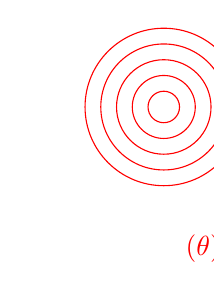
\begin{tikzpicture}
\TikzPlotArea{}
\TikzPtheta{blue}{$\p(\theta)$}

\onslide<2->{
\draw[red] (3, 1)  node[anchor=north] {$\qopt(\theta)$};
\foreach \s in {0.2, 0.4, 0.6, 0.8, 1.0}
    \draw[red] (2.5,2.5) ellipse (\s * 1 and \s * 1);
}
\end{tikzpicture}
\end{minipage}

\onslide<2->{
\begin{center}
\textbf{KL minimizers ``fit inside'' the second argument.}
\end{center}
}

\end{frame}




%%%%%%%%%%%%%%%%%%%%%%%%%%%%%%%%%%%%%%%%%%%%%%%%%%%%%%%%%%%%%%%%%%%%%%%%%%%%%%
%%%%%%%%%%%%%%%%%%%%%%%%%%%%%%%%%%%%%%%%%%%%%%%%%%%%%%%%%%%%%%%%%%%%%%%%%%%%%%
%%%%%%%%%%%%%%%%%%%%%%%%%%%%%%%%%%%%%%%%%%%%%%%%%%%%%%%%%%%%%%%%%%%%%%%%%%%%%%

\begin{frame}{KL divergence exercises}
\begin{minipage}{0.5\textwidth}
    %
\begin{align*}
%
\MoveEqLeft
\kl{\p(\theta)}{\q(\theta)} ={}\\&
-\expect{\p(\theta)}{\log \q(\theta)} +
\expect{\p(\theta)}{\log \p(\theta)}\\ \\
\p(\theta) ={}& \textrm{Correlated bivariate normal}\\ \\
%
\qdom ={}& \left\{ \textrm{Independent bivariate normals}\right\}\\ \\
%
\end{align*}
%
What is
$\qopt(\theta) ={} \argmin{\q \in \qdom} \kl{\p(\theta)}{\q(\theta)}$?
%
\end{minipage}
%
\begin{minipage}{0.4\textwidth}

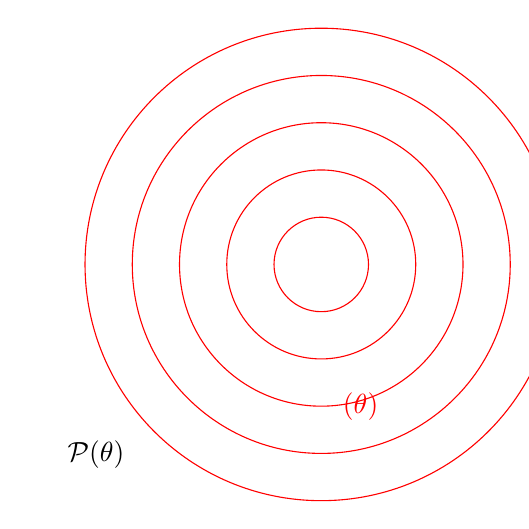
\begin{tikzpicture}
\TikzPlotArea{}
\TikzPtheta{blue}{$\p(\theta)$}

\onslide<2->{
\draw[red] (3, 1)  node[anchor=north] {$\qopt(\theta)$};
\foreach \s in {0.2, 0.4, 0.6, 0.8, 1.0}
    \draw[red] (2.5,2.5) ellipse (\s * 3 and \s * 3);
}
\end{tikzpicture}
\end{minipage}

\onslide<2->{
\begin{center}
\textbf{KL minimizers ``fit inside'' the second argument.}
\end{center}
}

\end{frame}




%%%%%%%%%%%%%%%%%%%%%%%%%%%%%%%%%%%%%%%%%%%%%%%%%%%%%%%%%%%%%%%%%%%%%%%%%%%%%%
%%%%%%%%%%%%%%%%%%%%%%%%%%%%%%%%%%%%%%%%%%%%%%%%%%%%%%%%%%%%%%%%%%%%%%%%%%%%%%
%%%%%%%%%%%%%%%%%%%%%%%%%%%%%%%%%%%%%%%%%%%%%%%%%%%%%%%%%%%%%%%%%%%%%%%%%%%%%%

\begin{frame}{KL divergence exercises}
\hspace{-3em}
\begin{minipage}{0.5\textwidth}
%
\begin{align*}
%
\MoveEqLeft
\kl{\q(\theta)}{\p(\theta)} ={}\\&
-\expect{\q(\theta)}{\log \p(\theta)} +
\expect{\q(\theta)}{\log \q(\theta)}\\ \\
\p(\theta) ={}& \textrm{Correlated bivariate normal}\\ \\
\qdom ={}& \left\{ \textrm{Bivariate normals}\right\}\\ \\
%
\end{align*}

What is $\qopt(\theta) = $\\
$\argmin{\q \in \qdom}
\Big(-\expect{\q(\theta)}{\log \p(\theta)} +$
\sout{$\expect{\q(\theta)}{\log \q(\theta)} \Big)$}?
%
\end{minipage}
%
\begin{minipage}{0.4\textwidth}

\begin{tikzpicture}
\TikzPlotArea{}
\TikzPtheta{blue}{$\p(\theta)$}

\onslide<2->{
\draw[red] (3, 1)  node[anchor=north] {$\qopt(\theta)$};
\node at (2.5,2.5) [circle,fill=red,inner sep=1.5pt]{};
}
\end{tikzpicture}
\end{minipage}

\onslide<2->{
\begin{center}
\textbf{Without the entropy, the KL minimizer concentrates on the
maximum of $\log \p(\theta)$.}
\end{center}
}

\end{frame}



%%%%%%%%%%%%%%%%%%%%%%%%%%%%%%%%%%%%%%%%%%%%%%%%%%%%%%%%%%%%%%%%%%%%%%%%%%%%%%
%%%%%%%%%%%%%%%%%%%%%%%%%%%%%%%%%%%%%%%%%%%%%%%%%%%%%%%%%%%%%%%%%%%%%%%%%%%%%%
%%%%%%%%%%%%%%%%%%%%%%%%%%%%%%%%%%%%%%%%%%%%%%%%%%%%%%%%%%%%%%%%%%%%%%%%%%%%%%

\begin{frame}{KL divergence exercises}
\hspace{-3em}
\begin{minipage}{0.5\textwidth}
%
\begin{align*}
%
\MoveEqLeft
\kl{\q(\theta)}{\p(\theta)} ={}\\&
-\expect{\q(\theta)}{\log \p(\theta)} +
\expect{\q(\theta)}{\log \q(\theta)}\\ \\
\p(\theta) ={}& \textrm{Correlated bivariate normal}\\ \\
\qdom ={}& \left\{ \textrm{Bivariate normals}\right\}\\ \\
%
\end{align*}

What is $\qopt(\theta) = $\\
$\argmin{\q \in \qdom} \Big(-$
\sout{$\expect{\q(\theta)}{\log \p(\theta)}$}
$+ \expect{\q(\theta)}{\log \q(\theta)} \Big)$?
%
\end{minipage}
%
\begin{minipage}{0.4\textwidth}

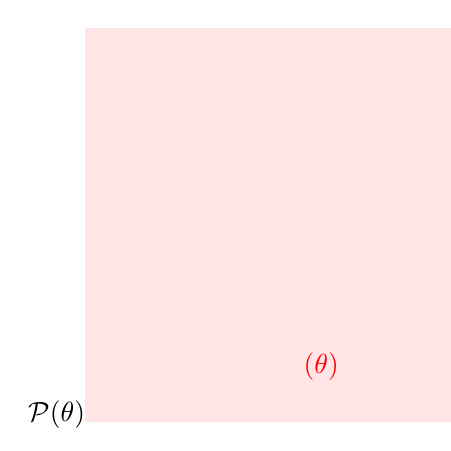
\begin{tikzpicture}
\TikzPlotArea{}
\TikzPtheta{blue}{$\p(\theta)$}

\onslide<2->{
\draw[red] (3, 1)  node[anchor=north] {$\qopt(\theta)$};
%\node at (2.5,2.5) [circle,fill=red,inner sep=1.5pt]{};
\draw[draw opacity=0, fill opacity=0.1, fill=red] (0,0) rectangle (5, 5);

}
\end{tikzpicture}
\end{minipage}

\onslide<2->{
\begin{center}
\textbf{Without $\log \p(\theta)$, the KL minimizer is infinitely dispersed.}
\end{center}
}

\end{frame}



%%%%%%%%%%%%%%%%%%%%%%%%%%%%%%%%%%%%%%%%%%%%%%%%%%%%%%%%%%%%%%%%%%%%%%%%%%%%%%
%%%%%%%%%%%%%%%%%%%%%%%%%%%%%%%%%%%%%%%%%%%%%%%%%%%%%%%%%%%%%%%%%%%%%%%%%%%%%%
%%%%%%%%%%%%%%%%%%%%%%%%%%%%%%%%%%%%%%%%%%%%%%%%%%%%%%%%%%%%%%%%%%%%%%%%%%%%%%

\begin{frame}{KL divergence exercises}
\hspace{-3em}
\begin{minipage}{0.5\textwidth}
%
\begin{align*}
%
\MoveEqLeft
\kl{\q(\theta)}{\p(\theta)} ={}\\&
-\expect{\q(\theta)}{\log \p(\theta)} +
\expect{\q(\theta)}{\log \q(\theta)}\\ \\
\p(\theta) ={}& \textrm{Correlated bivariate normal}\\ \\
\qdom ={}& \left\{ \textrm{Point masses}\right\}\\ \\
%
\end{align*}

What is $\qopt(\theta) ={} \argmin{\q \in \qdom} \kl{\q(\theta)}{\p(\theta)}$?
%
\end{minipage}
%
\begin{minipage}{0.4\textwidth}


\begin{tikzpicture}
\TikzPlotArea{}
\TikzPtheta{blue}{$\p(\theta)$}

\onslide<2->{
\draw[red] (2.5, 2.5)  node[anchor=north] {\texttt{UNDEFINED}};
%\node at (2.5,2.5) [circle,fill=red,inner sep=1.5pt]{};

}
\end{tikzpicture}
\end{minipage}

\onslide<2->{
\begin{center}
\textbf{Without a common dominating measure, the KL
divergence is undefined.}
\end{center}
}

\end{frame}




%%%%%%%%%%%%%%%%%%%%%%%%%%%%%%%%%%%%%%%%%%%%%%%%%%%%%%%%%%%%%%%%%%%%%%%%%%%%%%
%%%%%%%%%%%%%%%%%%%%%%%%%%%%%%%%%%%%%%%%%%%%%%%%%%%%%%%%%%%%%%%%%%%%%%%%%%%%%%
%%%%%%%%%%%%%%%%%%%%%%%%%%%%%%%%%%%%%%%%%%%%%%%%%%%%%%%%%%%%%%%%%%%%%%%%%%%%%%

\begin{frame}{KL divergence exercises}
\hspace{-3em}
\begin{minipage}{0.5\textwidth}
%
\begin{align*}
%
\MoveEqLeft
\kl{\q(\theta)}{\p(\theta)} ={}\\&
-\expect{\q(\theta)}{\log \p(\theta)} +
\expect{\q(\theta)}{\log \q(\theta)}\\ \\
\p(\theta) ={}& \textrm{Correlated bivariate normal}\\ \\
\qdom ={}& \left\{ \textrm{BVN with small, fixed variance}\right\}\\ \\
%
\end{align*}

What is $\qopt(\theta) ={} \argmin{\q \in \qdom} \kl{\q(\theta)}{\p(\theta)}$?
%
\end{minipage}
%
\begin{minipage}{0.4\textwidth}

\begin{tikzpicture}
\TikzPlotArea{}
\TikzPtheta{blue}{$\p(\theta)$}

\onslide<2->{
\draw[red] (3, 1)  node[anchor=north] {$\qopt(\theta)$};
\node at (2.5,2.5) [circle,fill=red,inner sep=1.5pt]{};
}
\end{tikzpicture}
\end{minipage}

\onslide<2->{
\begin{center}
\textbf{Sufficently concentrated distributions with constant entropy
act like a point mass at the maximum of $\log \p(\theta)$.}
\end{center}
}

\end{frame}



\newcommand{\TikzPtheta}[2]{
\draw[#1] (4.5, 3)  node[anchor=north] {#2};
\begin{scope}[shift={(2.5,2.5)}]
    \begin{scope}[rotate=45]
        \begin{scope}[shift={(-2.5,-2.5)}]
            \foreach \s in {0.2, 0.4, 0.6, 0.8, 1.0}
            \draw[#1] (2.5,2.5) ellipse (\s * 3 and \s * 1);
        \end{scope}
    \end{scope}
\end{scope}
}


\newcommand{\TikzPlotArea}{
\draw (0,0)--(5,0);
\foreach \x in {0,...,5}
  \draw (\x,0)--(\x,-.1) node[anchor=north]{};

\draw (0,0)--(0,5);
\foreach \y in {0,...,5}
  \draw (0,\y)--(-.1,\y) node[anchor=east] {};

\draw (0,5) node[anchor=east] {$\theta_2$};
\draw (5,0) node[anchor=north] {$\theta_1$};
}


%%%%%%%%%%%%%%%%%%%%%%%%%%%%%%%%%%%%%%%%%%%%%%%%%%%%%%%%%%%%%%%%%%%%%%%%%%%%%%
%%%%%%%%%%%%%%%%%%%%%%%%%%%%%%%%%%%%%%%%%%%%%%%%%%%%%%%%%%%%%%%%%%%%%%%%%%%%%%
%%%%%%%%%%%%%%%%%%%%%%%%%%%%%%%%%%%%%%%%%%%%%%%%%%%%%%%%%%%%%%%%%%%%%%%%%%%%%%

\begin{frame}{KL divergence exercises}
\begin{minipage}{0.5\textwidth}
%
\begin{align*}
%
\MoveEqLeft
\kl{\q(\theta)}{\p(\theta)} ={}\\&
-\expect{\q(\theta)}{\log \p(\theta)} +
\expect{\q(\theta)}{\log \q(\theta)}\\ \\
\p(\theta) ={}& \textrm{Correlated bivariate normal}\\ \\
%
\qdom ={}& \left\{ \textrm{All bivariate normals}\right\}\\ \\
%
\end{align*}
%
What is
$\qopt(\theta) = \argmin{\q \in \qdom} \kl{\q(\theta)}{\p(\theta)}$?
%
\end{minipage}
%
\begin{minipage}{0.4\textwidth}

\begin{tikzpicture}
\TikzPlotArea{}
\TikzPtheta{blue}{$\p(\theta)$}

\onslide<2->{
\TikzPtheta{red}{}
\draw[red] (4.5, 2.5)  node[anchor=north] {$\qopt(\theta)$};
}
\end{tikzpicture}
\end{minipage}

\onslide<2->{
\begin{center}
\textbf{Sufficiently expressive families recover the target distribution.}
\end{center}
}

\end{frame}


%%%%%%%%%%%%%%%%%%%%%%%%%%%%%%%%%%%%%%%%%%%%%%%%%%%%%%%%%%%%%%%%%%%%%%%%%%%%%%
%%%%%%%%%%%%%%%%%%%%%%%%%%%%%%%%%%%%%%%%%%%%%%%%%%%%%%%%%%%%%%%%%%%%%%%%%%%%%%
%%%%%%%%%%%%%%%%%%%%%%%%%%%%%%%%%%%%%%%%%%%%%%%%%%%%%%%%%%%%%%%%%%%%%%%%%%%%%%

\begin{frame}{KL divergence exercises}
\begin{minipage}{0.5\textwidth}
    %
\begin{align*}
%
\MoveEqLeft
\kl{\q(\theta)}{\p(\theta)} ={}\\&
-\expect{\q(\theta)}{\log \p(\theta)} +
\expect{\q(\theta)}{\log \q(\theta)}\\ \\
\p(\theta) ={}& \textrm{Correlated bivariate normal}\\ \\
%
\qdom ={}& \left\{ \textrm{Independent bivariate normals}\right\}\\ \\
%
\end{align*}
%
What is
$\qopt(\theta) = \argmin{\q \in \qdom} \kl{\q(\theta)}{\p(\theta)}$?
%
\end{minipage}
%
\begin{minipage}{0.4\textwidth}

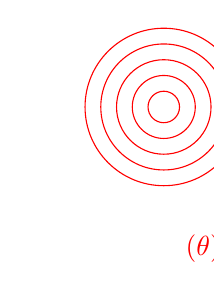
\begin{tikzpicture}
\TikzPlotArea{}
\TikzPtheta{blue}{$\p(\theta)$}

\onslide<2->{
\draw[red] (3, 1)  node[anchor=north] {$\qopt(\theta)$};
\foreach \s in {0.2, 0.4, 0.6, 0.8, 1.0}
    \draw[red] (2.5,2.5) ellipse (\s * 1 and \s * 1);
}
\end{tikzpicture}
\end{minipage}

\onslide<2->{
\begin{center}
\textbf{KL minimizers ``fit inside'' the second argument.}
\end{center}
}

\end{frame}




%%%%%%%%%%%%%%%%%%%%%%%%%%%%%%%%%%%%%%%%%%%%%%%%%%%%%%%%%%%%%%%%%%%%%%%%%%%%%%
%%%%%%%%%%%%%%%%%%%%%%%%%%%%%%%%%%%%%%%%%%%%%%%%%%%%%%%%%%%%%%%%%%%%%%%%%%%%%%
%%%%%%%%%%%%%%%%%%%%%%%%%%%%%%%%%%%%%%%%%%%%%%%%%%%%%%%%%%%%%%%%%%%%%%%%%%%%%%

\begin{frame}{KL divergence exercises}
\begin{minipage}{0.5\textwidth}
    %
\begin{align*}
%
\MoveEqLeft
\kl{\p(\theta)}{\q(\theta)} ={}\\&
-\expect{\p(\theta)}{\log \q(\theta)} +
\expect{\p(\theta)}{\log \p(\theta)}\\ \\
\p(\theta) ={}& \textrm{Correlated bivariate normal}\\ \\
%
\qdom ={}& \left\{ \textrm{Independent bivariate normals}\right\}\\ \\
%
\end{align*}
%
What is
$\qopt(\theta) ={} \argmin{\q \in \qdom} \kl{\p(\theta)}{\q(\theta)}$?
%
\end{minipage}
%
\begin{minipage}{0.4\textwidth}

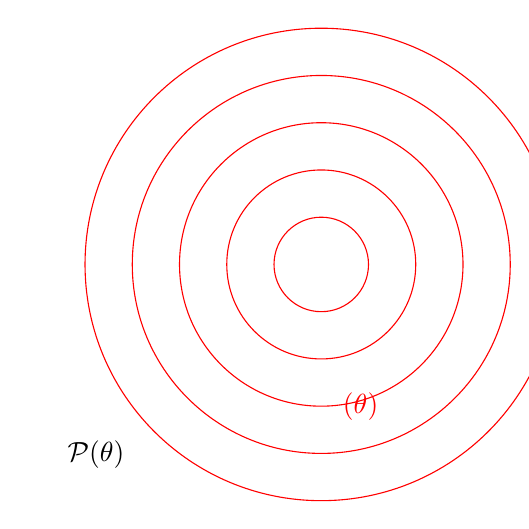
\begin{tikzpicture}
\TikzPlotArea{}
\TikzPtheta{blue}{$\p(\theta)$}

\onslide<2->{
\draw[red] (3, 1)  node[anchor=north] {$\qopt(\theta)$};
\foreach \s in {0.2, 0.4, 0.6, 0.8, 1.0}
    \draw[red] (2.5,2.5) ellipse (\s * 3 and \s * 3);
}
\end{tikzpicture}
\end{minipage}

\onslide<2->{
\begin{center}
\textbf{KL minimizers ``fit inside'' the second argument.}
\end{center}
}

\end{frame}




%%%%%%%%%%%%%%%%%%%%%%%%%%%%%%%%%%%%%%%%%%%%%%%%%%%%%%%%%%%%%%%%%%%%%%%%%%%%%%
%%%%%%%%%%%%%%%%%%%%%%%%%%%%%%%%%%%%%%%%%%%%%%%%%%%%%%%%%%%%%%%%%%%%%%%%%%%%%%
%%%%%%%%%%%%%%%%%%%%%%%%%%%%%%%%%%%%%%%%%%%%%%%%%%%%%%%%%%%%%%%%%%%%%%%%%%%%%%

\begin{frame}{KL divergence exercises}
\hspace{-3em}
\begin{minipage}{0.5\textwidth}
%
\begin{align*}
%
\MoveEqLeft
\kl{\q(\theta)}{\p(\theta)} ={}\\&
-\expect{\q(\theta)}{\log \p(\theta)} +
\expect{\q(\theta)}{\log \q(\theta)}\\ \\
\p(\theta) ={}& \textrm{Correlated bivariate normal}\\ \\
\qdom ={}& \left\{ \textrm{Bivariate normals}\right\}\\ \\
%
\end{align*}

What is $\qopt(\theta) = $\\
$\argmin{\q \in \qdom}
\Big(-\expect{\q(\theta)}{\log \p(\theta)} +$
\sout{$\expect{\q(\theta)}{\log \q(\theta)} \Big)$}?
%
\end{minipage}
%
\begin{minipage}{0.4\textwidth}

\begin{tikzpicture}
\TikzPlotArea{}
\TikzPtheta{blue}{$\p(\theta)$}

\onslide<2->{
\draw[red] (3, 1)  node[anchor=north] {$\qopt(\theta)$};
\node at (2.5,2.5) [circle,fill=red,inner sep=1.5pt]{};
}
\end{tikzpicture}
\end{minipage}

\onslide<2->{
\begin{center}
\textbf{Without the entropy, the KL minimizer concentrates on the
maximum of $\log \p(\theta)$.}
\end{center}
}

\end{frame}



%%%%%%%%%%%%%%%%%%%%%%%%%%%%%%%%%%%%%%%%%%%%%%%%%%%%%%%%%%%%%%%%%%%%%%%%%%%%%%
%%%%%%%%%%%%%%%%%%%%%%%%%%%%%%%%%%%%%%%%%%%%%%%%%%%%%%%%%%%%%%%%%%%%%%%%%%%%%%
%%%%%%%%%%%%%%%%%%%%%%%%%%%%%%%%%%%%%%%%%%%%%%%%%%%%%%%%%%%%%%%%%%%%%%%%%%%%%%

\begin{frame}{KL divergence exercises}
\hspace{-3em}
\begin{minipage}{0.5\textwidth}
%
\begin{align*}
%
\MoveEqLeft
\kl{\q(\theta)}{\p(\theta)} ={}\\&
-\expect{\q(\theta)}{\log \p(\theta)} +
\expect{\q(\theta)}{\log \q(\theta)}\\ \\
\p(\theta) ={}& \textrm{Correlated bivariate normal}\\ \\
\qdom ={}& \left\{ \textrm{Bivariate normals}\right\}\\ \\
%
\end{align*}

What is $\qopt(\theta) = $\\
$\argmin{\q \in \qdom} \Big(-$
\sout{$\expect{\q(\theta)}{\log \p(\theta)}$}
$+ \expect{\q(\theta)}{\log \q(\theta)} \Big)$?
%
\end{minipage}
%
\begin{minipage}{0.4\textwidth}

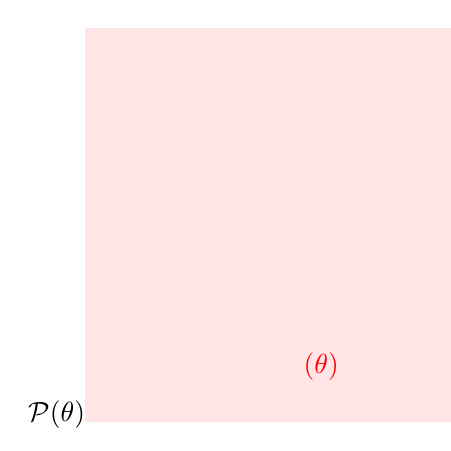
\begin{tikzpicture}
\TikzPlotArea{}
\TikzPtheta{blue}{$\p(\theta)$}

\onslide<2->{
\draw[red] (3, 1)  node[anchor=north] {$\qopt(\theta)$};
%\node at (2.5,2.5) [circle,fill=red,inner sep=1.5pt]{};
\draw[draw opacity=0, fill opacity=0.1, fill=red] (0,0) rectangle (5, 5);

}
\end{tikzpicture}
\end{minipage}

\onslide<2->{
\begin{center}
\textbf{Without $\log \p(\theta)$, the KL minimizer is infinitely dispersed.}
\end{center}
}

\end{frame}



%%%%%%%%%%%%%%%%%%%%%%%%%%%%%%%%%%%%%%%%%%%%%%%%%%%%%%%%%%%%%%%%%%%%%%%%%%%%%%
%%%%%%%%%%%%%%%%%%%%%%%%%%%%%%%%%%%%%%%%%%%%%%%%%%%%%%%%%%%%%%%%%%%%%%%%%%%%%%
%%%%%%%%%%%%%%%%%%%%%%%%%%%%%%%%%%%%%%%%%%%%%%%%%%%%%%%%%%%%%%%%%%%%%%%%%%%%%%

\begin{frame}{KL divergence exercises}
\hspace{-3em}
\begin{minipage}{0.5\textwidth}
%
\begin{align*}
%
\MoveEqLeft
\kl{\q(\theta)}{\p(\theta)} ={}\\&
-\expect{\q(\theta)}{\log \p(\theta)} +
\expect{\q(\theta)}{\log \q(\theta)}\\ \\
\p(\theta) ={}& \textrm{Correlated bivariate normal}\\ \\
\qdom ={}& \left\{ \textrm{Point masses}\right\}\\ \\
%
\end{align*}

What is $\qopt(\theta) ={} \argmin{\q \in \qdom} \kl{\q(\theta)}{\p(\theta)}$?
%
\end{minipage}
%
\begin{minipage}{0.4\textwidth}


\begin{tikzpicture}
\TikzPlotArea{}
\TikzPtheta{blue}{$\p(\theta)$}

\onslide<2->{
\draw[red] (2.5, 2.5)  node[anchor=north] {\texttt{UNDEFINED}};
%\node at (2.5,2.5) [circle,fill=red,inner sep=1.5pt]{};

}
\end{tikzpicture}
\end{minipage}

\onslide<2->{
\begin{center}
\textbf{Without a common dominating measure, the KL
divergence is undefined.}
\end{center}
}

\end{frame}




%%%%%%%%%%%%%%%%%%%%%%%%%%%%%%%%%%%%%%%%%%%%%%%%%%%%%%%%%%%%%%%%%%%%%%%%%%%%%%
%%%%%%%%%%%%%%%%%%%%%%%%%%%%%%%%%%%%%%%%%%%%%%%%%%%%%%%%%%%%%%%%%%%%%%%%%%%%%%
%%%%%%%%%%%%%%%%%%%%%%%%%%%%%%%%%%%%%%%%%%%%%%%%%%%%%%%%%%%%%%%%%%%%%%%%%%%%%%

\begin{frame}{KL divergence exercises}
\hspace{-3em}
\begin{minipage}{0.5\textwidth}
%
\begin{align*}
%
\MoveEqLeft
\kl{\q(\theta)}{\p(\theta)} ={}\\&
-\expect{\q(\theta)}{\log \p(\theta)} +
\expect{\q(\theta)}{\log \q(\theta)}\\ \\
\p(\theta) ={}& \textrm{Correlated bivariate normal}\\ \\
\qdom ={}& \left\{ \textrm{BVN with small, fixed variance}\right\}\\ \\
%
\end{align*}

What is $\qopt(\theta) ={} \argmin{\q \in \qdom} \kl{\q(\theta)}{\p(\theta)}$?
%
\end{minipage}
%
\begin{minipage}{0.4\textwidth}

\begin{tikzpicture}
\TikzPlotArea{}
\TikzPtheta{blue}{$\p(\theta)$}

\onslide<2->{
\draw[red] (3, 1)  node[anchor=north] {$\qopt(\theta)$};
\node at (2.5,2.5) [circle,fill=red,inner sep=1.5pt]{};
}
\end{tikzpicture}
\end{minipage}

\onslide<2->{
\begin{center}
\textbf{Sufficently concentrated distributions with constant entropy
act like a point mass at the maximum of $\log \p(\theta)$.}
\end{center}
}

\end{frame}


\begin{frame}{Conclusions}

\footnotesize

\bibliographystyle{plainnat}
% Hide the references header
% https://tex.stackexchange.com/questions/22645/hiding-the-title-of-the-bibliography/370784
\begingroup
\renewcommand{\section}[2]{}%
\bibliography{references}
\endgroup

\end{frame}


\end{document}
